% TEMPLATE.TEX
%
% Time-stamp: <2013-03-26 11:09 olenz>
%
% This is an extensively documented LaTeX file that shows how to
% produce a good-looking document with current LaTeX (11/2012).
%
% IMPORTANT!
%
%   Some obsolete commands and packages
% ----------|-------------------------------
% obsolete  |     Replacement in LATEX 2ε
% ----------|-------------------------------
%           | local            global/switch
% ----------|-------------------------------
% {\bf ...} | \textbf{...}     \bfseries
%     -     | \emph{...}       \em
% {\it ...} | \textit{...}     \itshape
%     -     | \textmd{...}     \mdseries
% {\rm ...} | \textrm{...}     \rmfamily
% {\sc ...} | \textsc{...}     \scshape
% {\sf ...} | \textsf{...}     \sffamily
% {\sl ...} | \textsl{...}     \slshape
% {\tt ...} | \texttt{...}     \ttfamily
%     -     | \textup{...}     \upshape
%
% DON'T USE \\ TO MAKE LINEBREAKS, INSTEAD JUST LEAVE A BLANK LINE!
%
\RequirePackage[l2tabu,orthodox]{nag} % turn on warnings because of bad style
\documentclass[a4paper,10pt,bibtotoc]{scrartcl}
%
\usepackage[bottom=3.5cm, top=3cm]{geometry}
\usepackage{subcaption}
\captionsetup[subfigure]{list=true, position=top}
\usepackage{float}
%%%%%%%%%%%%%%%%%%%%%%%%%%%%%%%%%%%%
% KOMA CLASSES
%%%%%%%%%%%%%%%%%%%%%%%%%%%%%%%%%%%%
%
% The class "scrartcl" is one of the so-called KOMA-classes, a set of
% very well done LaTeX-classes that produce a very European layout
% (e.g. titles with a sans-serif font).
%
% The KOMA classes have extensive documentation that you can access
% via the commands:
%   texdoc scrguide # in German
%   texdoc scrguien # in English
%
%
% The available classes are:
%
% scrartcl - for "articles", typically for up to ~20 pages, the
%            highest level sectioning command is \section
%
% scrreprt - for "reports", typically for up to ~200 pages, the
%            highest level sectioning command is \chapter
%
% scrbook  - for "books", for more than 200 pages, the highest level
%            sectioning command is \part.
%
% USEFUL OPTIONS
%
% a4paper  - Use a4 paper instead of the default american letter
%            format.
%
% 11pt, 12pt, 10pt
%          - Use a font with the given size.
%
% bibtotoc - Add the bibliography to the table of contents
%
% The KOMA-script classes have plenty of options to modify

% This allows to type UTF-8 characters like ä,ö,ü,ß
\usepackage[utf8]{inputenc}

\usepackage[T1]{fontenc}        % Tries to use Postscript Type 1 Fonts for better rendering
\usepackage{lmodern}            % Provides the Latin Modern Font which offers more glyphs than the default Computer Modern
\usepackage[intlimits]{amsmath} % Provides all mathematical commands
\usepackage{amssymb}
\usepackage{hyperref}           % Provides clickable links in the PDF-document for \ref
\usepackage{graphicx}            % Allow you to include images (like graphicx). Usage: \includegraphics{path/to/file}

% Allows to set units
\usepackage[ugly]{units}        % Allows you to type units with correct spacing and font style. Usage: $\unit[100]{m}$ or $\unitfrac[100]{m}{s}$

% Additional packages
\usepackage{url}                % Lets you typeset urls. Usage: \url{http://...}
\usepackage{breakurl}           % Enables linebreaks for urls
\usepackage{xspace}             % Use \xpsace in macros to automatically insert space based on context. Usage: \newcommand{\es}{ESPResSo\xspace}
\usepackage{xcolor}             % Obviously colors. Usage: \color{red} Red text
\usepackage{booktabs}           % Nice rules for tables. Usage \begin{tabular}\toprule ... \midrule ... \bottomrule
\usepackage{siunitx}


% Source code listings
\usepackage{listings}           % Source Code Listings. Usage: \begin{lstlisting}...\end{lstlisting}
\lstloadlanguages{python}
\definecolor{lightpurple}{rgb}{0.8,0.8,1}

\lstset{
stepnumber=1,
numbersep=5pt,
numberstyle=\small\color{black},
basicstyle=\ttfamily,
%keywordstyle=\color{black},
%commentstyle=\color{black},
%stringstyle=\color{black},
frame=single,
tabsize=4,
language = python,
backgroundcolor=\color{black!5}}

\usepackage{float}

\begin{document}

\titlehead{Simulation Methods in Physics I \hfill WS 2019/2010}
\title{Report for Worksheet 4: Thermostats}
\author{Markus Baur and David Beyer}
\date{\today}
%\publishers{Institute for Computational Physics, University of Stuttgart}
\maketitle

\tableofcontents

\section{Random Numbers}
\subsection{Linear Congruental Generator}
The code for this exercise can be found in the file ex\_4\_3\_random\_walk.py.
We implemented the linear congruental generator as a generator:
\begin{lstlisting}
def linear_congruental_generator():
    a = 1103515245
    c = 13245
    m = 2**32
    seed = 123647
    X = seed
    while True:
        X = (a*X + c) % m
        yield X/m
\end{lstlisting}
The declaration of the function as a generator allows us to use it as an iterator using the next command. 
In this case, the seed is just a fixed number (123647). Because we want a pseudo-random number in the interval $(0,1)$, the generator yields the quotient $X/m$.

To generate random walks consisting of $N$ steps starting from the starting point $x_0$, we wrote the following function:
\begin{lstlisting}
def random_walk(N, x0):
    ret = np.empty(N+1)
    ret[0] = x0
    k = linear_congruental_generator()
    for i in range(N):
        ret[i+1] = ret[i] + next(k) - 0.5
    return ret
\end{lstlisting}
This function has as its arguments the number of steps $N$ and the starting point $x_0$ and returns a NumPy array of length $N+1$ which contains the individual steps of the trajectory.
Every step, a random step size $\Delta x\in (-0.5,0.5)$ is added.
The random step size is generated using the function for the linear congruental generator defined above.
We could verify that the generated trajectory is always the same for a given seed.

To generate different trajectories, we use a different seed for every random walk.
One way to do this is to generate a seed from the current time:
\begin{lstlisting}
def linear_congruental_generator():
    a = 1103515245
    c = 13245
    m = 2**32
    seed = int(time.time()*10**7)
    X = seed
    while True:
        X = (a*X + c) % m
        yield X/m
\end{lstlisting}
A plot of ten different random walks which where generated using this method is shown in \autoref{fig:fig1}.
\begin{figure}[H]
	\centering
	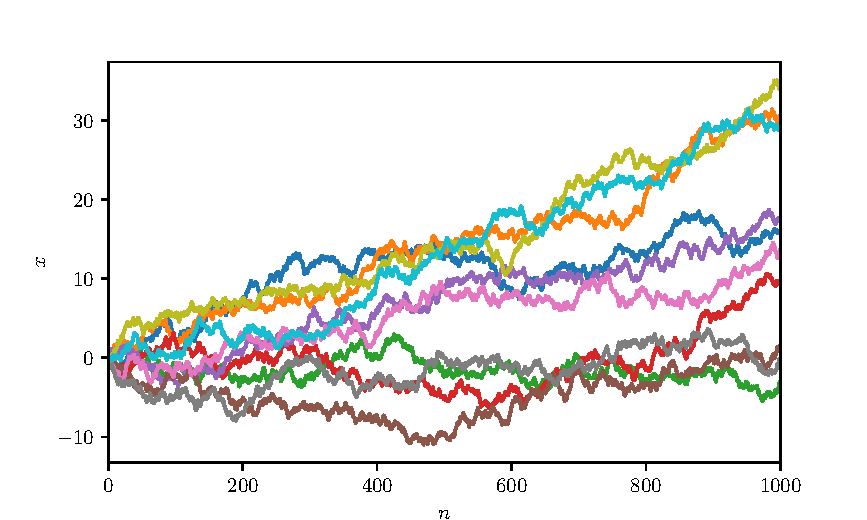
\includegraphics[width=\linewidth]{random_walk_time.pdf}
	\caption{Plot of ten different random walks with a seed generated from the current time.}
	\label{fig:fig1}
\end{figure}
\noindent Alternatively, we can create a random seed using os.urandom():
\begin{lstlisting}
def linear_congruental_generator():
    a = 1103515245
    c = 13245
    m = 2**32
    seed = int.from_bytes(os.urandom(10), sys.byteorder)
    X = seed
    while True:
        X = (a*X + c) % m
        yield X/m
\end{lstlisting}
A plot of ten different random walks which where generated using this method is shown in \autoref{fig:fig2}.
\begin{figure}[H]
	\centering
	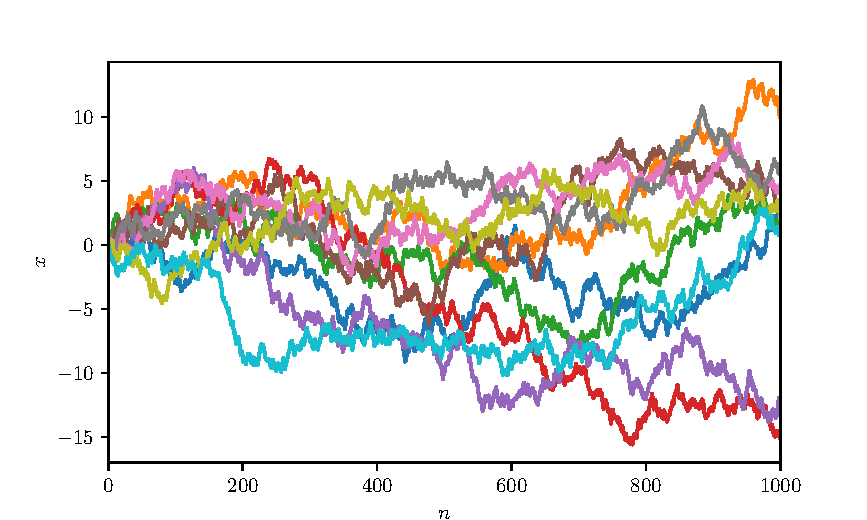
\includegraphics[width=\linewidth]{random_walk_os.pdf}
	\caption{Plot of ten different random walks with a seed generated using os.urandom().}
	\label{fig:fig2}
\end{figure}

\subsection{Box-Muller Transform}
\subsubsection{Gaussian Distribution}
The code for this exercise can be found in the file ex\_4\_3\_box\_muller.py. 
We again implemented a generator, it yields the random numbers which follow a Gaussian distribution and are generated using the Box-Muller transform:
\begin{lstlisting}
def box_muller(mean, sigma):
    while True:
        u1 = np.random.random()
        u2 = np.random.random()
        n1 = mean + sigma*np.sqrt(-2*np.log(u1))*np.cos(2*np.pi*u2)
        n2 = mean + sigma*np.sqrt(-2*np.log(u1))*np.sin(2*np.pi*u2)
        yield n1
        yield n2
\end{lstlisting}
The function has as its argument the desired mean and standard deviation of the Gaussian distribution. 
To generate the intial pair of random numbers, the NumPy implementation of the Mersenne Twister is used.
Then, the Box-Muller transform is performed.

A normalized histogram of $N=10000$ random numbers generated using the Box-Muller transform with mean of $\mu=1.0$ and standard deviation $\sigma = 4.0$ is shown in \autoref{fig:fig3}. 
Comparison with the analytical Gaussian distribution shows that the histogram approaches the analytical result quite closely.
\begin{figure}[H]
	\centering
	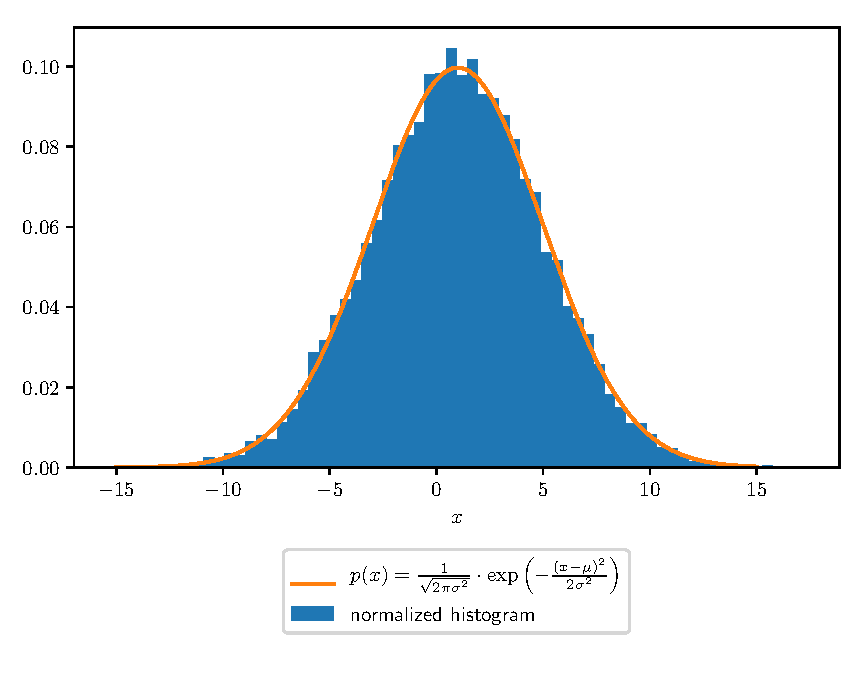
\includegraphics[width=\linewidth]{gaussian.pdf}
	\caption{Normalized histogram of $N=10000$ random numbers generated using the Box-Muller transform with mean of $\mu=1.0$ and standard deviation $\sigma = 4.0$. The analytical Gaussian distribution is also included.}
	\label{fig:fig3}
\end{figure}

\subsubsection{Maxwell-Boltzmann Distribution}
The distribution of particle speeds in a fluid can be described by the Maxwell-Boltzmann distribution.
To derive the Maxwell-Boltzmann distribution in three dimensions, we start with the canonical distribution for a classical fluid of $N$ particles, given by
\begin{align}
p\left(\{\mathbf{r}_i\}_{i=1,...,N},\{\mathbf{p}_i\}_{i=1,...,N}\right)\mathrm{d}\xi = \frac{1}{h^{3N}\cdot N!\cdot Z}\cdot\exp\left(-\beta\left(\sum_{i=1}^{N}\frac{\mathbf{p}_i^2}{2m} + V\left(\{\mathbf{r}_i\}_{i=1,...,N}\right)\right)\right)\mathrm{d}\xi.
\end{align}
Integrating over all particle coordinates results in the momentum distribution function
\begin{align}
p\left(\{\mathbf{p}_i\}_{i=1,...,N}\right)\mathrm{d}p = \mathcal{N}'\cdot\exp\left(-\beta\left(\sum_{i=1}^{N}\frac{\mathbf{p}_i^2}{2m} \right)\right)\mathrm{d}p
\end{align}
with a normalization $\mathcal{N}'$. 
Because the distribution factorizes and is the same for all particles, we may as well just look at the distribution of the $i$th particle, given by (we drop the index $i$):
\begin{align}
p\left(\mathbf{p}\right)\mathrm{d}p_x\mathrm{d}p_y\mathrm{d}p_z = \mathcal{N}\cdot\exp\left(-\beta\frac{\mathbf{p}^2}{2m}\right)\mathrm{d}p_x\mathrm{d}p_y\mathrm{d}p_z = \underbrace{\mathcal{N}m^3\cdot\exp\left(-\beta\frac{m\mathbf{v}^2}{2}\right)}_{=p\left(\mathbf{v}\right)}\mathrm{d}v_x\mathrm{d}v_y\mathrm{d}v_z.
\end{align}
$\mathcal{N}$ is again a normalization factor.
We can easily see that the individual components of the velocity are distributed according to a Gaussian distribution with mean $\mu= 0$ and standard deviation $\sigma = \left(\beta m\right)^{-\frac{1}{2}}$.
To obtain a distribution of the speed $v=\left|\mathbf{v}\right|$ we transform to spherical coordinates and integrate over the angles $\theta$ and $\phi$:
\begin{align}
\begin{split}
p\left(v\right)\mathrm{d}v &= \int_{\Omega}\,\mathcal{N}m^3\cdot\exp\left(-\beta\frac{mv^2}{2}\right)v^2\mathrm{d}v\mathrm{d}\Omega = 4\pi\mathcal{N}m^3v^2\cdot\exp\left(-\beta\frac{mv^2}{2}\right)\mathrm{d}v\\
&=\underbrace{4\pi\sqrt{\frac{\beta m}{2\pi}}^3v^2\cdot\exp\left(-\beta\frac{mv^2}{2}\right)}_{\text{Maxwell-Boltzmann distribution}}\mathrm{d}v.
\end{split}
\end{align}
Because the velocity components follow a Gaussian distribution, we can produce a Maxwell-Boltzmann distribution by calculating the distribution of the absolute values of threedimensional vectors with components that follow a Gaussian distribution.
Using the box\_muller generator defined above, this can be done in the following way:
\begin{lstlisting}
random_velocites = box_muller(0.0, 1.0)
v = [np.array([next(random_velocites),next(random_velocites),\
     next(random_velocites)]) for i in range(N_velocities)] 
v = np.array(v)
\end{lstlisting}

\begin{figure}[H]
	\centering
	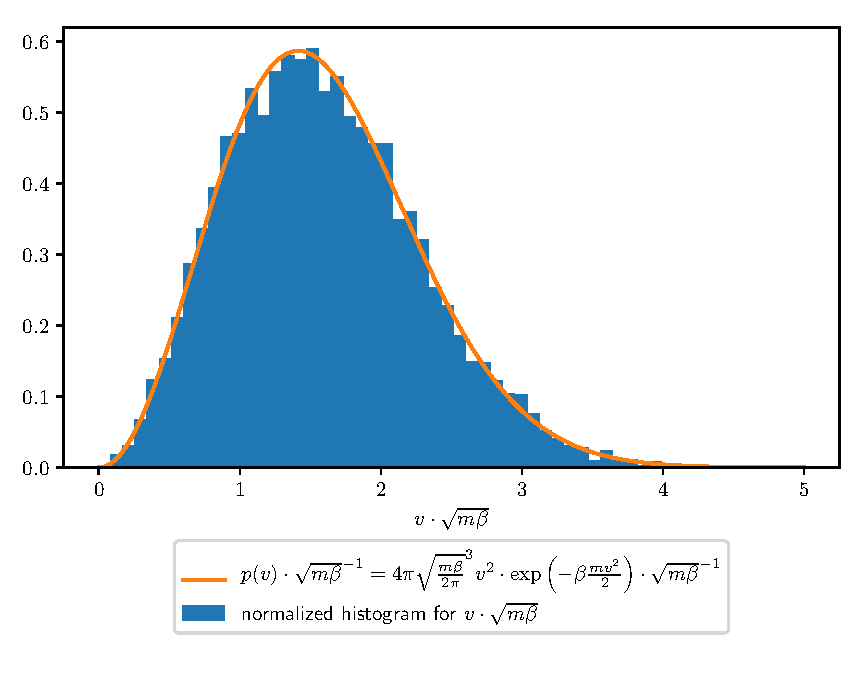
\includegraphics[width=\linewidth]{maxwell_boltzmann.pdf}
	\caption{Normalized histogram for the absolute value of $N=1000$ random 3-vectors $\mathbf{v}$ whose components are distributed according to a Gaussian distribution with mean $\mu=0.0$ and standard deviation $\sigma = 1.0$. The analytical Maxwell-Boltzmann distribution is also plotted.}
	\label{fig:fig4}
\end{figure}

\section{Langevin thermostat}
\section{Diffusion coefficients}
\section{Diffusion equation}
      
\end{document}
